\documentclass[lettersize,journal]{IEEEtran}

% ---------------------------------------------------------------
% Packages
% ---------------------------------------------------------------
\usepackage{amsmath,amssymb}
\usepackage{graphicx}
\usepackage{booktabs}
\usepackage{multirow}
\usepackage{hyperref}
\usepackage{cite}
\usepackage{array}
\usepackage{stfloats}
\usepackage{url}
\usepackage{tikz}
\usetikzlibrary{shapes.geometric, arrows.meta, positioning,
                fit, backgrounds, calc}

\hyphenation{op-tical net-works semi-conduc-tor IEEE-Xplore}

% ---------------------------------------------------------------
\begin{document}
% ---------------------------------------------------------------

\title{Regime-Aware Multi-Head Deep Q-Network\\
       for Adaptive Traffic Signal Control}

\author{Suraj~Meruva,~\IEEEmembership{Student~Member,~IEEE,}
        and~Boini~Abhiram,~\IEEEmembership{Student~Member,~IEEE}%
\thanks{Manuscript received ; revised .}%
\thanks{S.~Meruva and B.~Abhiram are with the Department of Data Science and
Artificial Intelligence, Indian Institute of Information Technology, Naya
Raipur, Chhattisgarh, India.}}

\maketitle

% ---------------------------------------------------------------
\begin{abstract}
Traffic lights are hard to get right, because traffic itself keeps changing:
a quiet road at midnight and a jammed one at rush hour call for very
different decisions. This paper tells the story of how we built and tested a
Traffic-Regime Aware Multi-Head Deep Q-Network (MH-DQN) -- a traffic-signal
controller that learns to recognize which kind of traffic it is looking at
and reacts accordingly. We built it up in five stages, each one a little more
realistic than the last. We start small, with a standard DQN controlling one
ordinary four-way intersection, just to prove the idea works. From there, we
add the regime-aware, multi-head design; scale it up to a synthetic
3 $\times$ 3 grid of nine intersections; and finally hand it the keys to a
real six-junction road corridor, modeled in SUMO from an actual street in
Hyderabad. At every stage, we compare our controller against the kind of
fixed-time signal already used in the real world today: one that simply
gives 30 seconds of green to north--south traffic, then 30 seconds to
east--west traffic, on repeat, no matter how much traffic is actually there.
On the single intersection, our controller cuts average waiting time by
73.53\% and average queue length by 41.69\% compared to that fixed-time
baseline. Moving it straight to the real-world corridor, without any further
training, still cuts waiting time by 49.5\%, but throughput drops by 33\% --
a trade-off worth fixing. So we fine-tune it, adjusting how heavily it is
penalized for switching phases too often. After 100 fine-tuning episodes, the
corridor-deployed controller cuts average waiting time by 40.2\%, queue
length by 28.2\%, and raises average speed by 5.1\%, while throughput falls
by only 11.0\% under a realistic peak demand of 2,000 vehicles per hour.
Taken together, these results show that teaching a controller to recognize
different traffic regimes, and to specialize its behavior for each one, is a
strategy that keeps working as we move from a single toy intersection to a
grid of nine, and finally to a real, messy, six-junction road network.
\end{abstract}

\begin{IEEEkeywords}
Adaptive Traffic Signal Control, Road transportation, Reinforcement Learning, Intelligent networked transportation systems
\end{IEEEkeywords}

% ---------------------------------------------------------------
\section{Introduction}
\label{sec:intro}
% ---------------------------------------------------------------

\IEEEPARstart{A}{nyone} who has sat at a red light while the cross street stays
empty knows that traffic signals do not always match the traffic in front of
them. This mismatch is not just an annoyance -- at the scale of a whole city,
it wastes fuel, adds to emissions, and eats away at people's
time~\cite{wei2018intellilight,liang2019deep}. Most signals today still run on
a fixed-time plan: a timer that hands out green light on a repeating schedule,
regardless of how many cars are actually waiting. That approach is simple and
reliable, but it cannot adapt when traffic surges, thins out, or shifts
direction.

Reinforcement learning (RL) offers a different way forward. Instead of
following a fixed schedule, an RL agent learns its own signal-timing policy by
interacting with a traffic environment and gradually discovering what works
best~\cite{mnih2015human}. Because it treats signal control as a sequence of
decisions rather than a static plan, it can pick up strategies that a
hand-designed schedule would never find, especially once the traffic
situation grows complex or unpredictable.

Even so, most RL-based signal controllers still make one simplifying
assumption: a single network is trained to handle every traffic condition at
once. That assumption misses something important about real streets, shown in
Fig.~\ref{fig:traffic_regimes}: traffic does not behave the same way at all
times. A nearly empty road, a moderately busy one, and a fully jammed one each
call for a different style of control. A single policy can learn to do
reasonably well on average, but it tends to fall short of what a policy
tailored to each of these regimes could achieve~\cite{chu2020multiagent}.

% ------------------------------------------------------------------
% FIGURE 1 — TikZ traffic regimes diagram (no image file needed)
% ------------------------------------------------------------------
\begin{figure}[!t]
\centering
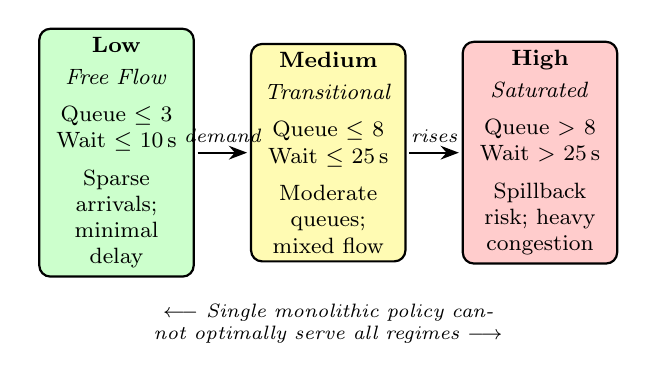
\begin{tikzpicture}[
    regime/.style={
        rectangle, rounded corners=4pt, draw=black, thick,
        text width=1.75cm, align=center, minimum height=2.4cm,
        font=\footnotesize, inner sep=3pt
    },
    arrow/.style={->, thick, >=Stealth,
                  shorten >=1pt, shorten <=1pt},
    lbl/.style={font=\scriptsize\itshape}
]
\node[regime, fill=green!20] (low) {
    \textbf{Low}\\[2pt]\textit{Free Flow}\\[4pt]
    Queue $\leq 3$\\Wait $\leq 10$\,s\\[4pt]
    Sparse arrivals; minimal delay};
\node[regime, fill=yellow!30, right=0.7cm of low] (med) {
    \textbf{Medium}\\[2pt]\textit{Transitional}\\[4pt]
    Queue $\leq 8$\\Wait $\leq 25$\,s\\[4pt]
    Moderate queues; mixed flow};
\node[regime, fill=red!20, right=0.7cm of med] (high) {
    \textbf{High}\\[2pt]\textit{Saturated}\\[4pt]
    Queue $> 8$\\Wait $> 25$\,s\\[4pt]
    Spillback risk; heavy congestion};
\draw[arrow] (low.east) -- node[above,lbl]{demand} (med.west);
\draw[arrow] (med.east) -- node[above,lbl]{rises}  (high.west);
\node[font=\scriptsize\itshape, align=center, below=0.4cm of med,
      text width=7.4cm]
    {$\longleftarrow$ Single monolithic policy cannot optimally
     serve all regimes $\longrightarrow$};
\end{tikzpicture}
\caption{Three traffic regimes at a signalized intersection. Each one comes
with its own typical queue length and waiting time, and so calls for its own
control strategy. A single policy cannot serve all three equally well, which
is why this paper proposes a multi-head architecture instead.}
\label{fig:traffic_regimes}
\end{figure}

In short, here is what this paper contributes:
\begin{itemize}
    \item A full, step-by-step build-up, starting from a standard DQN
          (Stage~1), adding multi-head specialization (Stage~2), scaling to a
          multi-agent grid (Stage~3), and finally moving to a real-world
          corridor through transfer (Stage~4) and fine-tuning (Stage~5).
    \item The MH-DQN architecture itself: one shared encoder feeding into
          several Q-heads, each specialized for a different traffic regime,
          coordinated by a regime classifier with soft gating.
    \item A close look at the trade-off between throughput and waiting time
          at every stage, along with the fine-tuning steps that ease it.
    \item Evidence that this approach transfers to a real six-junction
          arterial corridor, cutting waiting time by 40.2\% under a peak
          demand of 2{,}000~veh/hr.
\end{itemize}

% ---------------------------------------------------------------
\section{Related Work}
\label{sec:related}
% ---------------------------------------------------------------

\subsection{Adaptive Traffic Signal Control}

Researchers have been looking for alternatives to rigid fixed-time signals for
a long time. Classical systems such as SCOOT[] and SCATS[] were an early step:
they read detector measurements and look up the right response in a
pre-computed table, adjusting signal splits and offsets on the fly. That is
already an improvement over a static plan, but the rules are still hand-built
by engineers, so they do not generalize well to new traffic patterns or
unfamiliar road layouts. Later systems added detector-triggered green
extensions and decentralized, pressure-based heuristics, which react faster
but are still fundamentally reactive: the underlying control law is fixed in
advance and cannot reshape itself as demand changes across a day or a season.
Model-based approaches such as integer programming and model predictive
control take a more mathematical route and come with theoretical guarantees,
but they do not scale well and need an accurate traffic model that is hard to
keep up to date in the real world~\cite{liang2019deep}. Model predictive
controllers, in particular, must solve a fresh optimization problem at every
single decision step, and their performance drops sharply once the model
drifts away from real conditions -- a common problem in dense city traffic,
where lane discipline is loose and turning patterns shift constantly. These
shortcomings are what push the field toward data-driven, learning-based
controllers: ones that learn directly from experience instead of relying on a
hand-built model of the road network.

\subsection{Reinforcement Learning for Traffic Signal Control}

Deep reinforcement learning has become the leading data-driven alternative to
these older methods. Mnih et al.~\cite{mnih2015human} first showed that DQN
can handle complex sequential decision tasks well, and that result laid the
groundwork for almost all the RL-based signal-control work that followed. Wei
et al.~\cite{wei2018intellilight} put DQN to work directly on traffic signals
with IntelliLight, and found that a learned policy beats a fixed-time
controller at a single intersection -- though getting it to scale to a
network of junctions proved harder. Liang et al.~\cite{liang2019deep} improved
convergence with a phase-sensitive reward function, but still trained one
unified policy to handle every demand level.

Other work has pushed on the learning algorithm itself rather than the
traffic problem: Double DQN~\cite{hasselt2016deep} fixes a tendency to
overestimate values, and Dueling DQN~\cite{wang2016dueling} improves
stability, though both still rely on one monolithic policy. Prioritized
experience replay~\cite{schaul2016prioritized} speeds up learning by
replaying the transitions the network gets most wrong more often, and this
kind of improvement sits comfortably alongside architectural changes like
ours rather than competing with them. Looking beyond a single intersection,
multi-agent RL~\cite{chu2020multiagent} scales up by training one agent per
junction independently, while max-pressure control~\cite{wei2019presslight}
builds queue imbalance directly into the state so the network stays stable as
a whole. Transfer learning~\cite{mannion2018transfer} takes representations
learned in one setting and reuses them in a new one, cutting down how much
retraining is needed. Mixture-of-experts models~\cite{jacobs1991adaptive} have
separately shown that a set of specialized sub-networks can beat a single
monolithic one when the input naturally falls into different modes -- exactly
the situation multi-regime traffic presents. Recent surveys of the
field~\cite{haydari2022deep} catalogue a fast-growing variety of state
designs, reward functions, and coordination schemes, but they keep arriving at
the same observation: most deployed agents still lean on a single value
network and expect it to cover everything from an empty road to a fully
saturated one. Table~\ref{tab:related} lays out these approaches side by side
along with what each one leaves unsolved. The framework proposed here is
built to close exactly that gap: a regime-aware controller for intelligent
networked transportation systems that does not force one policy to do
everything at once.


\begin{table}[!t]
\caption{Summary of Key RL-Based TSC Approaches\label{tab:related}}
\centering
\renewcommand{\arraystretch}{1.25}
\begin{tabular}{@{}>{\raggedright}p{1.55cm}
                    >{\raggedright}p{1.85cm}
                    >{\raggedright\arraybackslash}p{3.35cm}@{}}
\toprule
\textbf{Author/Year} & \textbf{Approach} & \textbf{Limitation} \\
\midrule
Mnih et al.\ 2015~\cite{mnih2015human}
  & DQN with experience replay \& target network
  & Not traffic-specific; single monolithic policy \\
Wei et al.\ 2018~\cite{wei2018intellilight}
  & IntelliLight: DQN for single-intersection TSC
  & Single intersection only; no multi-regime handling \\
Liang et al.\ 2019~\cite{liang2019deep}
  & DRL with phase-sensitive reward shaping
  & Single unified policy \\
Hasselt et al.\ 2016~\cite{hasselt2016deep}
  & Double DQN (reduces overestimation)
  & Monolithic policy; no regime specialization \\
Wang et al.\ 2016~\cite{wang2016dueling}
  & Dueling DQN (value + advantage streams)
  & Monolithic; not evaluated for multi-junction networks \\
Chu et al.\ 2020~\cite{chu2020multiagent}
  & Multi-agent DRL for large-scale TSC
  & No traffic regime awareness \\
Mannion et al.\ 2018~\cite{mannion2018transfer}
  & Transfer learning for multi-intersection TSC
  & Single unified policy transferred; no regime specialization \\
\bottomrule
\end{tabular}
\end{table}

% ---------------------------------------------------------------
\section{System Architecture and Methodology}
\label{sec:arch}
% ---------------------------------------------------------------

We built this system step by step rather than all at once. It starts with a
standard DQN proving the concept on a single four-way intersection, then
grows through multi-head specialization, multi-agent grid scaling, and
finally real-world corridor deployment with fine-tuning. Building it this way
lets us check that each stage actually works before relying on it in the
next, so that any improvement we see can be traced back to the specific
change that produced it. Fig.~\ref{fig:system_overview} shows the general
architecture and information flow that all five stages share.

% ------------------------------------------------------------------
% FIGURE 2 — TikZ generic system overview (no image file needed)
% ------------------------------------------------------------------
\begin{figure}[!t]
\centering
\resizebox{\columnwidth}{!}{%
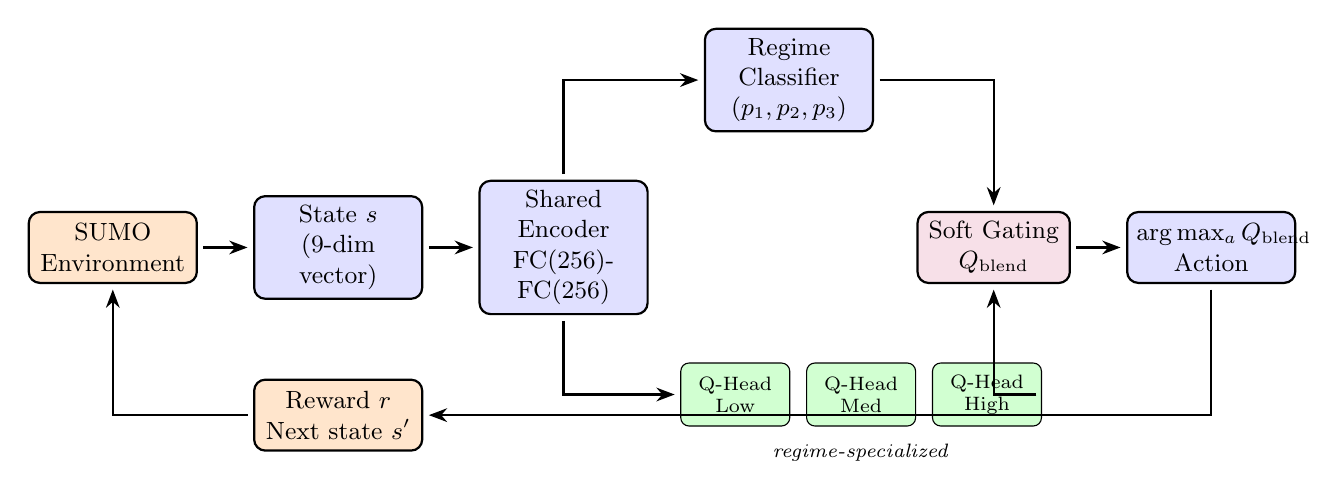
\begin{tikzpicture}[
    mainbox/.style={rectangle, draw=black, thick, rounded corners=4pt,
        fill=blue!12, text width=1.9cm, align=center,
        minimum height=0.9cm, font=\small},
    envbox/.style={rectangle, draw=black, thick, rounded corners=4pt,
        fill=orange!20, text width=1.9cm, align=center,
        minimum height=0.9cm, font=\small},
    headbox/.style={rectangle, draw=black, rounded corners=3pt,
        fill=green!18, text width=1.15cm, align=center,
        minimum height=0.8cm, font=\scriptsize},
    gatebox/.style={rectangle, draw=black, thick, rounded corners=4pt,
        fill=purple!12, text width=1.7cm, align=center,
        minimum height=0.9cm, font=\small},
    arrow/.style={->, thick, >=Stealth,
                  shorten >=2pt, shorten <=2pt}
]
% main horizontal pipeline
\node[envbox]  (env)   {SUMO\\Environment};
\node[mainbox, right=0.7cm of env]   (state) {State $s$\\(9-dim vector)};
\node[mainbox, right=0.7cm of state] (enc)
    {Shared\\Encoder\\FC(256)-FC(256)};
% classifier above, heads below
\node[mainbox, above right=0.6cm and 0.7cm of enc] (cls)
    {Regime\\Classifier\\$(p_1,p_2,p_3)$};
\node[headbox, below right=0.6cm and 0.4cm of enc] (qL) {Q-Head\\Low};
\node[headbox, right=0.2cm of qL] (qM) {Q-Head\\Med};
\node[headbox, right=0.2cm of qM] (qH) {Q-Head\\High};
% gate aligned with encoder, to the right of classifier/heads
\node[gatebox, right=3.4cm of enc] (gate)
    {Soft Gating\\$Q_{\text{blend}}$};
\node[mainbox, right=0.7cm of gate] (act)
    {$\arg\max_a Q_{\text{blend}}$\\Action};
\node[envbox, below=1.0cm of state] (rew)
    {Reward $r$\\Next state $s'$};
% arrows
\draw[arrow] (env)   -- (state);
\draw[arrow] (state) -- (enc);
\draw[arrow] (enc) |- (cls.west);
\draw[arrow] (enc) |- (qL.west);
\draw[arrow] (cls.east) -| (gate.north);
\draw[arrow] (qH.east)  -| (gate.south);
\draw[arrow] (gate) -- (act);
\draw[arrow] (act.south) |- (rew.east);
\draw[arrow] (rew.west)  -| (env.south);
\node[font=\scriptsize, below=0.1cm of qM]
    {\textit{regime-specialized}};
\end{tikzpicture}}
\caption{How information flows through the MH-DQN system, the same way in
all five stages. The SUMO environment produces a 9-dimensional state, which
the shared trunk encodes. The regime classifier turns that into soft
weights; the three specialized Q-heads compute a Q-value for each regime;
soft gating blends them into $Q_{\text{blend}}$; and the resulting greedy
action is sent back to the environment, which returns the next state and a
reward.}
\label{fig:system_overview}
\end{figure}

\subsection{Overall Development Pipeline}

Table~\ref{tab:stages} summarizes the five stages we moved through to build
this system. Each one builds directly on top of the last.

\begin{table}[!t]
\caption{Summary of Five Development Stages\label{tab:stages}}
\centering
\renewcommand{\arraystretch}{1.2}
\begin{tabular}{@{}c >{\raggedright}p{1.5cm}
                    >{\raggedright\arraybackslash}p{2.2cm} c@{}}
\toprule
\textbf{St.} & \textbf{Name} & \textbf{Environment} & \textbf{Ep.} \\
\midrule
1 & Basic DQN            & Single 4-way           & 200 \\
2 & MH-DQN               & Single 4-way           & 200 \\
3 & Grid Network         & $3\times3$ (9 junc.)   & 200 \\
4 & Habsiguda (transfer) & 6-junction corridor    & 100 \\
5 & Habsiguda (tuned)    & 6-junction corridor    & 100 \\
\bottomrule
\end{tabular}
\end{table}

\textbf{Why these episode budgets?}
Stages~1--3 each get 200 training episodes because the agents start from
scratch ($\epsilon$ decays from 1.0 to 0.05) and need enough time exploring to
encounter the full range of queue and demand conditions. Stages~4 and~5, by
contrast, get only 100 episodes each, because they are fine-tuning rather than
learning from zero: every junction agent starts from the weights already
trained in Stage~2, which already understand queue dynamics reasonably well.
Training much longer than 100 episodes would risk washing out those
useful, general representations -- a classic case of catastrophic
forgetting.

\subsection{Problem Formulation}

We treat adaptive traffic signal control as a Markov decision process (MDP)
$(S, A, P, R, \gamma)$ -- the standard way of describing a problem where an
agent takes actions, sees the results, and tries to do better over time.
Here is what each piece means in our setting.

\textbf{State space $S$:} what the agent sees at each moment.
\[
s = [\underbrace{q_N, q_S, q_E, q_W}_{\text{queue counts}},\;
     \underbrace{w_N, w_S, w_E, w_W}_{\text{waiting times}},\;
     \underbrace{\phi}_{\text{phase}}]
\]
The four queue counts tell the agent how many cars are backed up on each
approach; the four waiting times tell it how urgent each queue is; and the
phase value tells it which light is currently green. Together these nine
numbers are enough to tell what regime the traffic is in, how urgent the
situation is, and whether switching phases is worth it -- while staying small
enough for the network to train on smoothly.

\textbf{Action space $A$:} at every junction, the agent picks between just
two options: $a=0$ turns the north--south direction green, and $a=1$ turns
the east--west direction green.

\textbf{Transition dynamics $P$:} how the state changes when the agent acts.
$P(s'\mid s,a)$ depends on random vehicle arrivals and how SUMO routes them
through the network, so there is no clean formula for it. The agent never
sees this function directly -- it only learns from the
$(s,a,r,s')$ transitions it experiences and stores in a replay buffer.

\textbf{Reward function $R$:} the signal that tells the agent whether it did
well or poorly.
\begin{equation}
\label{eq:reward}
r = -0.1\,\text{wait} - 0.1\,\text{queue}
    + 1.0\,\text{throughput} - \lambda\,\text{phase\_change}
\end{equation}
Long waits and long queues are penalized, moving vehicles through is
rewarded, and $\lambda$ discourages switching phases too often
($\lambda=0.05$ in Stages~1--4; $\lambda=1.0$ in Stage~5).

\textbf{Discount factor $\gamma$:} how much the agent cares about the future
versus the present. We use $\gamma=0.99$ in Stage~1 (the standard DQN) and
$\gamma=0.95$ in Stages~2--5 (the MH-DQN). The slightly lower value in later
stages leans the agent toward relieving congestion sooner rather than later,
which also keeps training stable once the reward has multiple competing
goals and the traffic regime keeps switching.

\subsection{Multi-Head DQN Architecture}

The MH-DQN has three parts that work closely together, shown in full in
Fig.~\ref{fig:mhdqn_arch}.

\textbf{1) Shared State Encoder.}
Every Q-head and the regime classifier all draw on the same trunk: two
fully-connected layers of 256 units each, with ReLU activations. Sharing this
trunk keeps the total parameter count much lower than training three fully
separate networks, stops the heads from re-learning the same basic features
over and over, and pays off later when we transfer the model: the encoder
weights learned in Stage~2 are reused directly in Stages~4 and~5.

\textbf{2) Multiple Q-Heads.}
Sitting on top of the encoder are three Q-value networks (128 units, ReLU,
with a linear output of size $|A|=2$), one for each traffic regime:
\begin{itemize}
    \item \textbf{Low-regime head ($\theta_1$):} handles queue $\leq 3$ and
          wait $\leq 10$\,s. It learns not to switch phases needlessly when
          traffic is light and free-flowing.
    \item \textbf{Medium-regime head ($\theta_2$):} handles queue $\leq 8$
          and wait $\leq 25$\,s. It learns a balanced timing that clears
          moderate queues without leaving any approach waiting too long.
    \item \textbf{High-regime head ($\theta_3$):} handles queue $>8$ or
          wait $>25$\,s. It learns to clear queues aggressively so delays
          don't cascade once traffic is saturated.
\end{itemize}
Each head keeps its own parameters $\theta_k$ and its own target network
$\theta_k^{-}$, so the three regimes can specialize fully without their
training signals interfering with one another.

\textbf{3) Traffic Regime Classifier and Soft Gating.}
A small classifier network ($128\to64\to3$, softmax) reads the encoder's
output and estimates how likely the current state is to belong to each
regime, giving probabilities $(p_1,p_2,p_3)$; it is trained alongside the
Q-heads rather than separately. In Stages~1--2 we use \emph{hard switching}:
whichever regime scores highest ($\arg\max_k p_k$) is the only one that gets
to act. From Stage~4 onward we switch to \emph{soft gating}, which blends all
three heads together instead of picking just one:
\begin{equation}
\label{eq:blend}
Q_{\text{blend}}(s,a) = \sum_{k=1}^{K} p_k(s)\cdot Q(s,a;\,\theta_k)
\end{equation}
This matters a lot once we move to the multi-junction corridor, where traffic
drifts continuously between regimes rather than jumping cleanly from one to
another. Hard switching at a regime boundary causes the policy to lurch
abruptly, which shows up as erratic phase switching. Soft gating avoids this
by blending the Q-values in proportion to how confident the classifier is,
producing a smooth mix of the regime-specific policies instead of a jarring
handoff. This is exactly why the phase-change ratio keeps shrinking as the
stages progress: $2.32\times$ (Stage~2, hard switching) $\to$ $1.57\times$
(Stage~4) $\to$ $1.23\times$ (Stage~5).

% ------------------------------------------------------------------
% FIGURE 3 — TikZ detailed MH-DQN architecture (no image file needed)
% ------------------------------------------------------------------
\begin{figure}[!t]
\centering
\resizebox{\columnwidth}{!}{%
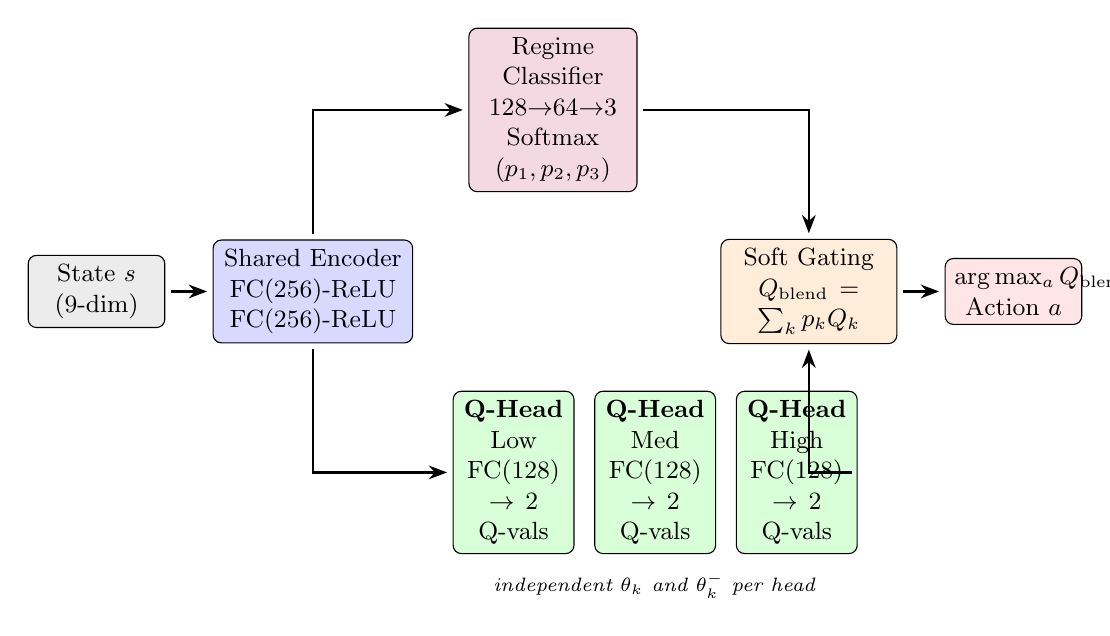
\begin{tikzpicture}[
    inputbox/.style={rectangle,draw,fill=gray!15,rounded corners=3pt,
        text width=1.5cm,align=center,minimum height=0.8cm,font=\small},
    encbox/.style={rectangle,draw,fill=blue!15,rounded corners=3pt,
        text width=2.3cm,align=center,minimum height=0.9cm,font=\small},
    clsbox/.style={rectangle,draw,fill=purple!15,rounded corners=3pt,
        text width=1.9cm,align=center,minimum height=1.0cm,font=\small},
    headbox/.style={rectangle,draw,fill=green!15,rounded corners=3pt,
        text width=1.3cm,align=center,minimum height=1.3cm,font=\small},
    gatebox/.style={rectangle,draw,fill=orange!15,rounded corners=3pt,
        text width=2.0cm,align=center,minimum height=1.0cm,font=\small},
    actbox/.style={rectangle,draw,fill=red!10,rounded corners=3pt,
        text width=1.5cm,align=center,minimum height=0.8cm,font=\small},
    arrow/.style={->,thick,>=Stealth,shorten >=2pt,shorten <=2pt}
]
\node[inputbox] (inp) {State $s$\\(9-dim)};
\node[encbox, right=0.6cm of inp] (enc)
    {Shared Encoder\\FC(256)-ReLU\\FC(256)-ReLU};
% classifier above encoder-right, heads below
\node[clsbox, above right=0.6cm and 0.7cm of enc] (cls)
    {Regime\\Classifier\\$128{\to}64{\to}3$\\Softmax\\$(p_1,p_2,p_3)$};
\node[headbox, below right=0.6cm and 0.5cm of enc] (qL)
    {\textbf{Q-Head}\\Low\\FC(128)\\$\to 2$ Q-vals};
\node[headbox, right=0.25cm of qL] (qM)
    {\textbf{Q-Head}\\Med\\FC(128)\\$\to 2$ Q-vals};
\node[headbox, right=0.25cm of qM] (qH)
    {\textbf{Q-Head}\\High\\FC(128)\\$\to 2$ Q-vals};
% gate to the right, between classifier and heads vertically
\node[gatebox, right=3.9cm of enc] (gate)
    {Soft Gating\\$Q_{\text{blend}}=\sum_k p_k Q_k$};
\node[actbox, right=0.6cm of gate] (act)
    {$\arg\max_a Q_{\text{blend}}$\\Action $a$};
\draw[arrow] (inp) -- (enc);
\draw[arrow] (enc) |- (cls.west);
\draw[arrow] (enc) |- (qL.west);
\draw[arrow] (cls.east) -| (gate.north);
\draw[arrow] (qH.east)  -| (gate.south);
\draw[arrow] (gate) -- (act);
\node[font=\scriptsize, below=0.12cm of qM]
    {\textit{independent $\theta_k$ and $\theta_k^{-}$ per head}};
\end{tikzpicture}}
\caption{A closer look at the MH-DQN architecture. The shared encoder pulls
out a common feature representation. The regime classifier turns that into
soft weights $(p_1,p_2,p_3)$. Three independent Q-heads -- each with its own
parameters $\theta_k$ and target network $\theta_k^{-}$ -- produce
regime-specific Q-values, which soft gating then blends into
$Q_{\text{blend}}$. The greedy action is simply whichever one maximizes
$Q_{\text{blend}}$.}
\label{fig:mhdqn_arch}
\end{figure}

\subsection{Training Objective}

We train the network using temporal difference (TD)
learning~\cite{mnih2015human}, the standard way of teaching a Q-network to
predict long-term value. Each Q-head $k$ is trained on its own, by trying to
shrink the squared TD error:
\begin{equation}
\label{eq:td}
\mathcal{L}(\theta_k) = \mathbb{E}\!\left[\!\left(
    \underbrace{r + \gamma\max_{a'}Q(s',a';\,\theta_k^{-})}_{\text{TD target (fixed)}}
    -\;\underbrace{Q(s,a;\,\theta_k)}_{\text{current prediction}}
\right)^{\!2}\right]
\end{equation}
In plain terms: $Q(s,a;\theta_k)$ is what the network currently predicts;
$r$ is the reward it just received, from~\eqref{eq:reward}; $\gamma$ is the
discount factor; and $\max_{a'}Q(s',a';\theta_k^{-})$ is its best guess at
the value of what comes next, computed by a separate target network
$\theta_k^{-}$. That target network is just a periodically-refreshed copy of
$\theta_k$ (synced every 100 steps), and keeping it separate stops the
network from chasing a moving target.

All three Q-heads draw from the same replay buffer of past experience, but
each keeps its own parameters $\theta_k$ and target network $\theta_k^{-}$.
We train with Adam (learning rate $10^{-3}$ for Stages~1--3, dropping to
$5\times10^{-5}$ for the fine-tuning in Stages~4--5) and $\epsilon$-greedy
exploration that decays from 1.0 to 0.05 (from 0.3 to 0.05 during
fine-tuning).

% ---------------------------------------------------------------
\section{Stage 1 --- Baseline Standard DQN}
\label{sec:stage1}
% ---------------------------------------------------------------

\subsection{Environment and Architecture}

Stage~1 is where we prove the basic idea works, using a standard DQN on a
simulated four-way signalized intersection. The network is simple:
Input(9)$\to$FC(128)$\to$FC(128)$\to$Output(2). Each episode sees 1{,}850
vehicles arrive at random. We train for 200 episodes, with $\epsilon$ decaying
from 1.0 to 0.05, a learning rate of $0.0001$, and $\gamma=0.99$. We compare
against a fixed-time baseline of 30\,s NS / 30\,s EW.

% ------------------------------------------------------------------
% FIGURE 4 — SUMO snapshot Stages 1 & 2   IMAGE: stage1&2.png
% ------------------------------------------------------------------
\begin{figure}[!t]
\centering
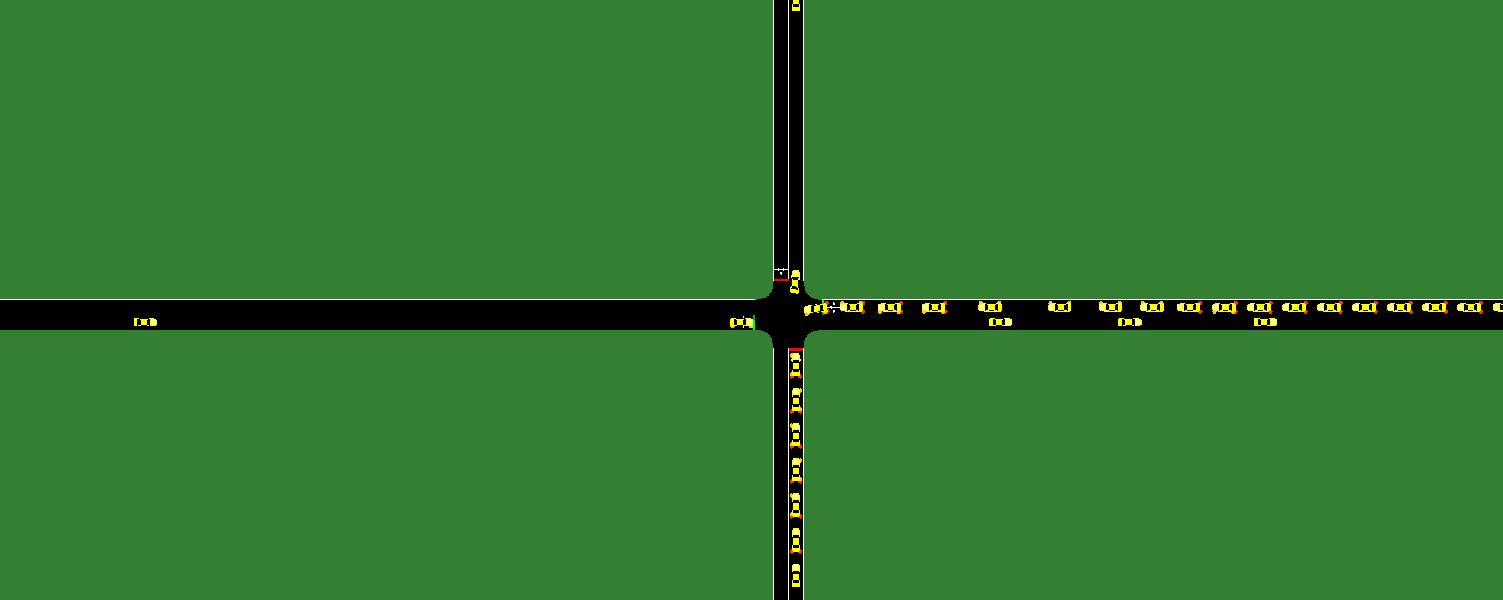
\includegraphics[width=3.4in]{stage1&2.png}
\caption{A snapshot from SUMO of the single four-way intersection used in
Stages~1 and~2. The yellow vehicles queued on the southbound and eastbound
approaches show a high-demand moment that the agent has to learn to clear.}
\label{fig:sim_stage12}
\end{figure}

\subsection{Key Observations}

This baseline DQN clearly beat random behavior, but it also exposed two
problems that pushed us toward the multi-head design: first, one policy
struggled to do its best across the whole range of traffic conditions within
a single episode; and second, we had to keep hand-tuning the reward to
balance throughput against congestion. Both observations are exactly what
led us to the regime-aware architecture in Stage~2.

% ---------------------------------------------------------------
\section{Stage 2 --- Multi-Head DQN (Single Intersection)}
\label{sec:stage2}
% ---------------------------------------------------------------

\subsection{Simulation Environment}

Stage~2 uses the same four-way intersection as Stage~1
(Fig.~\ref{fig:sim_stage12}), but swaps the standard DQN for the full
MH-DQN. During training, the regime classifier routes each experience to the
Q-head it belongs to; during inference, it blends the heads together
instead.

\subsection{Results}

Table~\ref{tab:results_sim} lays out the comparison. The MH-DQN cuts average
waiting time by 73.53\% (0.24\,s vs.\ 0.92\,s) and average queue length by
41.69\% (2.21 vs.\ 3.79). The cost is a 12.89\% drop in throughput, driven by
more frequent phase changes (253.3 vs.\ 109.0).

\begin{table}[!t]
\caption{MH-DQN vs.\ Fixed-Time Baseline
         (Stage~2, Single Intersection)\label{tab:results_sim}}
\centering
\renewcommand{\arraystretch}{1.2}
\begin{tabular}{@{}lcc@{}}
\toprule
\textbf{Metric} & \textbf{MH-DQN} & \textbf{Fixed-Time} \\
\midrule
Avg Reward          & $1095.78 \pm 11.97$ & $1253.46$ \\
Avg Wait Time (s)   & $\mathbf{0.24 \pm 0.02}$ & $0.92$ \\
Throughput (veh/hr) & $1129.78 \pm 12.42$ & $1297.00$ \\
Avg Queue Length    & $\mathbf{2.21 \pm 0.16}$ & $3.79$ \\
Vehicles Completed  & $1129.9$ & $1297.0$ \\
Phase Changes       & $253.3$  & $109.0$  \\
\bottomrule
\end{tabular}
\end{table}

% ------------------------------------------------------------------
% FIGURE 5 — Bar comparison Stage 2
% IMAGE: WhatsApp Image 2026-02-10 at 11.03.58 AM.jpeg
% ------------------------------------------------------------------
\begin{figure*}[!t]
\centering
\includegraphics[width=6.8in]{"WhatsApp Image 2026-02-10 at 11.03.58 AM.jpeg"}
\caption{MH-DQN vs.\ fixed-time baseline, compared side by side across six
metrics (Stage~2, single intersection).}
\label{fig:comparison}
\end{figure*}

% ------------------------------------------------------------------
% FIGURE 6 — Episode-by-episode comparison Stage 2
% IMAGE: WhatsApp Image 2026-02-10 at 11.03.54 AM.jpeg
% ------------------------------------------------------------------
\begin{figure}[!t]
\centering
\includegraphics[width=3.4in]{"WhatsApp Image 2026-02-10 at 11.03.54 AM.jpeg"}
\caption{Reward, waiting time, and throughput tracked episode by episode
over 10 evaluation episodes (Stage~2).}
\label{fig:episodes}
\end{figure}

% ------------------------------------------------------------------
% FIGURE 7 — Distribution Stage 2
% IMAGE: WhatsApp Image 2026-02-10 at 11.03.52 AM.jpeg
% ------------------------------------------------------------------
\begin{figure}[!t]
\centering
\includegraphics[width=3.4in]{"WhatsApp Image 2026-02-10 at 11.03.52 AM.jpeg"}
\caption{How episode rewards, waiting time, and throughput are distributed
(Stage~2, single intersection).}
\label{fig:distribution}
\end{figure}

% ------------------------------------------------------------------
% FIGURE 8 — Regime distribution Stage 2
% IMAGE: WhatsApp Image 2026-02-10 at 9.05.32 AM.jpeg
% ------------------------------------------------------------------
\begin{figure}[!t]
\centering
\includegraphics[width=3.4in]{"WhatsApp Image 2026-02-10 at 9.05.32 AM.jpeg"}
\caption{The traffic regimes seen during training turn out fairly balanced
across low, medium, and high demand (Stage~2).}
\label{fig:regime}
\end{figure}

Fig.~\ref{fig:comparison} shows this visually. Looking at the regime
distribution during training (Fig.~\ref{fig:regime}), the agent spent 32\%
of its time in the low regime, 41.8\% in the medium regime, and 26.2\% in
the high regime. During evaluation, the regime classifier gets every single
classification right -- 100\% accuracy (Fig.~\ref{fig:confusion}). The heads
also grow more distinct from one another as training goes on
(Fig.~\ref{fig:specialization}), confirming that each one really has learned
its own policy.

% ------------------------------------------------------------------
% FIGURE 9 — Confusion matrix training Stage 2
% IMAGE: WhatsApp Image 2026-02-10 at 9.05.37 AM.jpeg
% ------------------------------------------------------------------
\begin{figure}[!t]
\centering
\includegraphics[width=3.4in]{"WhatsApp Image 2026-02-10 at 9.05.37 AM.jpeg"}
\caption{How the regime classifier's predictions compare to the true
regimes during training (Stage~2, single intersection).}
\label{fig:confusion_train}
\end{figure}

% ------------------------------------------------------------------
% FIGURE 10 — Confusion matrix evaluation Stage 2
% IMAGE: WhatsApp Image 2026-02-10 at 10.48.34 AM.jpeg
% ------------------------------------------------------------------
\begin{figure}[!t]
\centering
\includegraphics[width=3.4in]{"WhatsApp Image 2026-02-10 at 10.48.34 AM.jpeg"}
\caption{The same comparison during evaluation, where the classifier gets
every regime right -- 100\% accuracy (Stage~2).}
\label{fig:confusion}
\end{figure}

% ------------------------------------------------------------------
% FIGURE 11 — Training dynamics Stage 2
% IMAGE: WhatsApp Image 2026-02-10 at 9.05.24 AM.jpeg
% ------------------------------------------------------------------
\begin{figure}[!t]
\centering
\includegraphics[width=3.4in]{"WhatsApp Image 2026-02-10 at 9.05.24 AM.jpeg"}
\caption{How training unfolds over 200 episodes: episode rewards, Q-loss,
classifier loss, waiting time, and classifier accuracy (Stage~2).}
\label{fig:training}
\end{figure}

% ------------------------------------------------------------------
% FIGURE 12 — Head specialization Stage 2
% IMAGE: WhatsApp Image 2026-02-10 at 9.05.42 AM.jpeg
% ------------------------------------------------------------------
\begin{figure}[!t]
\centering
\includegraphics[width=3.4in]{"WhatsApp Image 2026-02-10 at 9.05.42 AM.jpeg"}
\caption{How the head specialization score grows across training episodes,
showing the heads' policies pulling apart from each other (Stage~2).}
\label{fig:specialization}
\end{figure}

\subsection{Regime-Specific Performance}

Mean rewards stay consistent across all three regimes (0.37--0.39), which is
a good sign: it means each Q-head is doing its job well within its own
regime, not just getting lucky on the easy cases:
\begin{itemize}
    \item \textbf{Low:}    Mean reward = 0.37, Std = 0.57 (8{,}029 states)
    \item \textbf{Medium:} Mean reward = 0.39, Std = 0.59 (12{,}515 states)
    \item \textbf{High:}   Mean reward = 0.38, Std = 0.59 (7{,}852 states)
\end{itemize}

% ---------------------------------------------------------------
\section{Stage 3 --- Grid Network (Nine Intersections)}
\label{sec:stage3}
% ---------------------------------------------------------------

\subsection{Environment and Motivation}

Stage~3 asks a harder question: does this approach still work once there
are several intersections to manage at once? We test it on a synthetic
$3\times3$ grid of nine signalized junctions in SUMO. Each junction runs its
own independent MH-DQN agent, using the same Stage~2 architecture, the same
9-dimensional state, and the same 2-action space -- with no communication
between the agents at all. We train for 200 episodes.

% ------------------------------------------------------------------
% FIGURE 13 — 3×3 grid SUMO layout    IMAGE: stage3.png
% ------------------------------------------------------------------
\begin{figure}[!t]
\centering
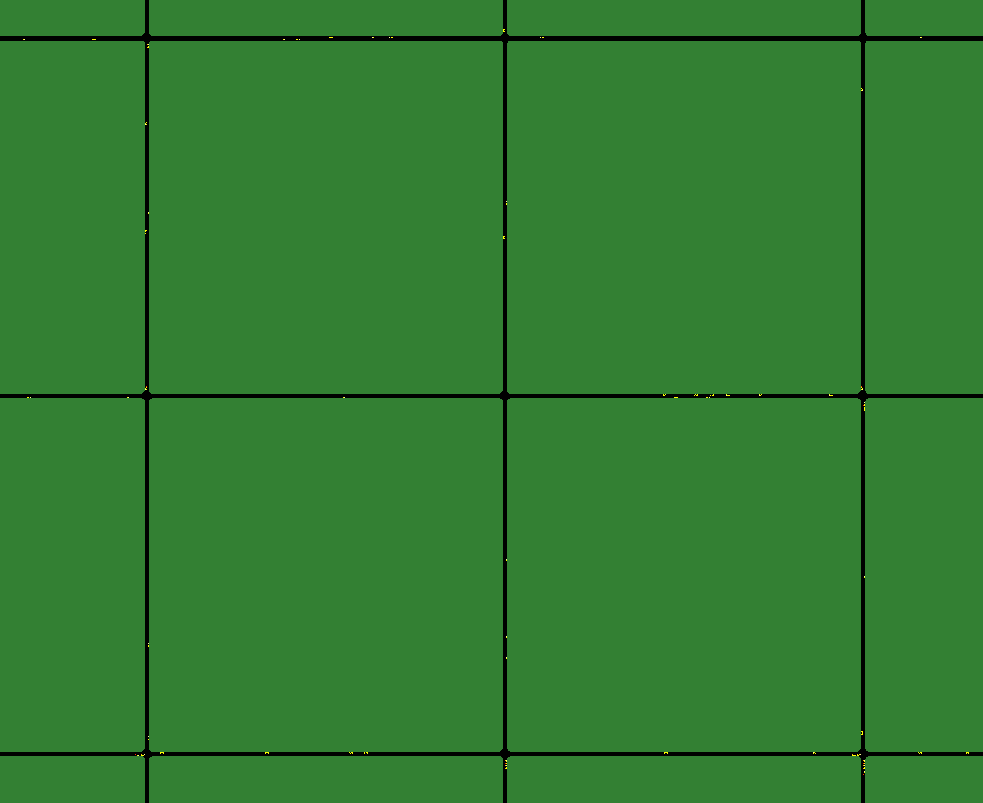
\includegraphics[width=3.4in]{stage3.png}
\caption{The synthetic $3\times3$ grid used in Stage~3, laid out in SUMO
with nine signalized intersections. Each cell is a road block bounded by
junctions; the grid shape is what lets us test how well decentralized
multi-agent control scales.}
\label{fig:sim_stage3}
\end{figure}

\subsection{Results}

Table~\ref{tab:grid} tracks how training progressed. Reward climbed from
$-629$ (Ep.~1) to a best of $-441.5$ (Ep.~113), and throughput grew by 4.3\%
from early to late training. Notably, the coordination score stayed at 0.0
throughout -- proof that the junctions did not need to talk to each other
directly for the grid as a whole to be managed well. That is an encouraging
sign for scaling this approach up further.

\begin{table}[!t]
\caption{Training Progression: $3\times3$ Grid (Stage~3)\label{tab:grid}}
\centering
\renewcommand{\arraystretch}{1.2}
\begin{tabular}{@{}lrr@{}}
\toprule
\textbf{Episode Block} & \textbf{Avg Reward} & \textbf{Throughput (veh/hr)} \\
\midrule
Ep.\ 1--10       & $-565.7$ & $467.2$ \\
Ep.\ 100         & $-503.7$ & $473.9$ \\
Ep.\ 190--200    & $-485.3$ & $487.3$ \\
\midrule
Best (Ep.\ 113)  & $-441.5$ & ---     \\
Worst (Ep.\ 1)   & $-628.7$ & ---     \\
\bottomrule
\end{tabular}
\end{table}

\subsection{Key Observations}

Stage~3 confirmed that this approach scales to multiple agents, but it also
surfaced a new problem: when each junction switches phases on its own
schedule, throughput can bottleneck right where junctions meet. That is what
led us to introduce the stronger phase-change penalty used in Stage~5.

% ---------------------------------------------------------------
\section{Stage 4 --- Real-World Corridor: Direct Transfer}
\label{sec:stage4}
% ---------------------------------------------------------------

\subsection{Corridor Environment and SUMO Modeling}

Now we leave the synthetic grids behind and test on a real street: the
Habsiguda--Nacharam corridor in Hyderabad, India, modeled in
SUMO~\cite{lopez2018microscopic}. As Fig.~\ref{fig:corridor_map} shows, it
runs about 3.9\,km along the Nacharam--Mallapur Road and passes through six
junctions:
\begin{itemize}
    \item J0: Habsiguda Junction (T-junction, corridor entry)
    \item J1: Habsiguda Colony Junction (four-way)
    \item J2: Nagendra Nagar Junction (four-way)
    \item J3: ECIL X Roads (four-way)
    \item J4: Nacharam X Roads (four-way)
    \item J5: Mallapur Junction (T-junction, corridor exit)
\end{itemize}

% ------------------------------------------------------------------
% FIGURE 14 — Corridor SUMO layout    IMAGE: stage4&5.png
% ------------------------------------------------------------------
\begin{figure}[!t]
\centering
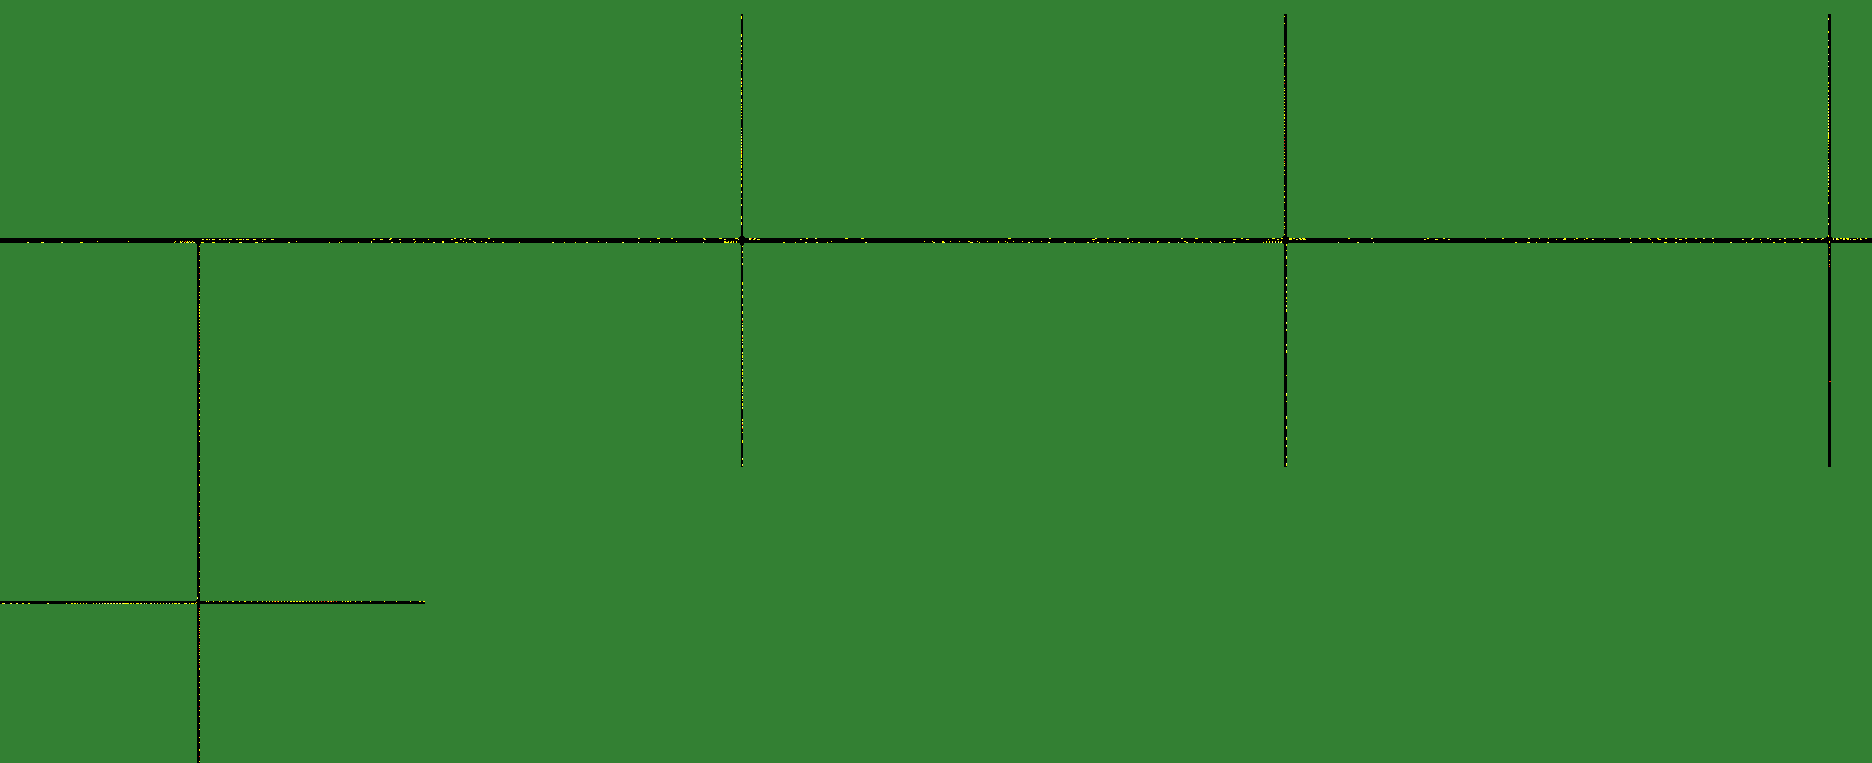
\includegraphics[width=3.4in]{stage4&5.png}
\caption{The six-junction corridor used in Stages~4 and~5, as laid out in
SUMO. The main road runs horizontally, with side roads branching off at
each of the six signalized junctions (J0--J5). Its uneven, asymmetric shape
comes straight from the real-world geometry of the corridor.}
\label{fig:sim_stage45}
\end{figure}

% ------------------------------------------------------------------
% FIGURE 15 — Real-world map          IMAGE: habsiguda_map.png
% ------------------------------------------------------------------
\begin{figure}[!t]
\centering
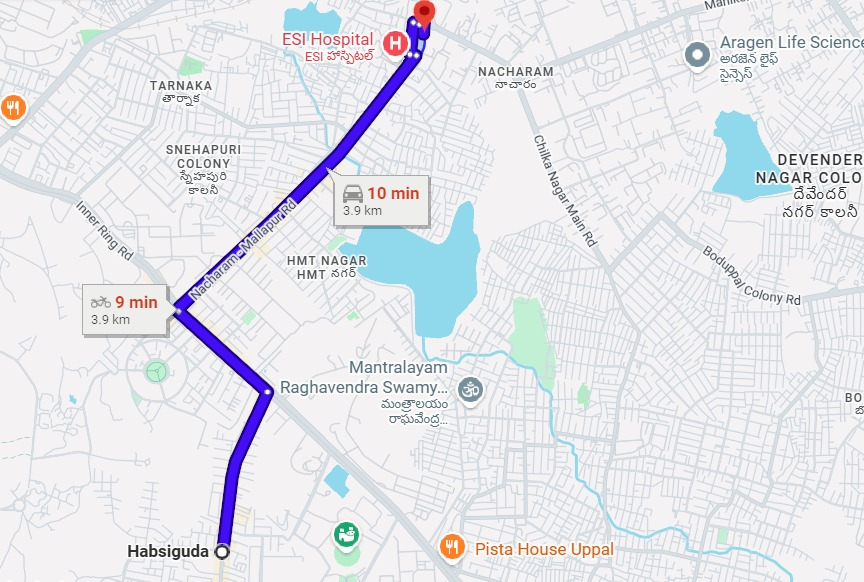
\includegraphics[width=3.4in]{habsiguda_map.png}
\caption{The real-world corridor we modeled in SUMO for Stages~4 and~5: a
3.9\,km stretch of road running from J0 to J5.}
\label{fig:corridor_map}
\end{figure}

We set traffic demand at 2{,}000~vehicles/hour, a realistic peak load. The
fixed-time baseline runs a 30\,s/30\,s cycle at every junction (450 phase
changes per episode), matching how the corridor is actually signaled today.

\subsection{Transfer Learning Setup}

For this stage, we take the MH-DQN agents straight from their Stage~2
pre-trained weights, with no retraining from scratch, and run them with: a
learning rate of $0.00005$, $\epsilon$ decaying from $0.3$ to $0.05$, 100
episodes, a phase penalty of $\lambda=0.05$, and a minimum green time of
10\,s.

\subsection{Results}

Table~\ref{tab:results_hab4} shows what happens when the model is dropped
straight into the real corridor. It performs well on waiting time
($-49.5\%$) and queue length ($-35.1\%$), just as it did before. But
throughput takes a real hit, falling $-33.0\%$ -- nearly three times what we
saw at the single intersection. The cause is not hard to find: without a
strong enough phase-change penalty, the agents switch phases far too often
(705.2 vs.\ 450.0 in the baseline), and every extra switch means another
all-red period where nothing moves. This is exactly the problem Stage~5's
fine-tuning sets out to fix.

\begin{table}[!t]
\caption{Direct Transfer MH-DQN vs.\ Fixed-Time
         (Stage~4)\label{tab:results_hab4}}
\centering
\renewcommand{\arraystretch}{1.2}
\begin{tabular}{@{}lccc@{}}
\toprule
\textbf{Metric} & \textbf{Fixed} & \textbf{MH-DQN} & \textbf{Change} \\
\midrule
Throughput (veh/hr) & 945.5 & 633.3            & $-33.0\%$ \\
Vehicles Completed  & 946.0 & 633.6            & $-33.0\%$ \\
Avg Wait Time (s)   & 3.11  & $\mathbf{1.57}$  & $\mathbf{-49.5\%}$ \\
Avg Queue Length    & 77.03 & $\mathbf{50.03}$ & $\mathbf{-35.1\%}$ \\
Phase Changes       & 450.0 & 705.2            & $+56.7\%$ \\
\bottomrule
\end{tabular}
\end{table}

% ---------------------------------------------------------------
\section{Stage 5 --- Fine-Tuned MH-DQN (Real-World Corridor)}
\label{sec:stage5}
% ---------------------------------------------------------------

\subsection{Fine-Tuning Protocol and Reward Adjustments}

To fix the throughput problem from Stage~4, we make two targeted changes to
the reward, shown in Table~\ref{tab:reward_changes}. As before, all six
junction agents start from Stage~2's pre-trained weights, and we fine-tune
them for 100 episodes. The best reward reached during fine-tuning is
$-357.57$.

\begin{table}[!t]
\caption{Reward Parameter Changes: Stage~4 vs.\ Stage~5%
\label{tab:reward_changes}}
\centering
\renewcommand{\arraystretch}{1.2}
\begin{tabular}{@{}lcc@{}}
\toprule
\textbf{Parameter}        & \textbf{Stage~4} & \textbf{Stage~5} \\
\midrule
Min Green Time            & 10\,s   & \textbf{20\,s} \\
Phase Penalty $\lambda$   & $0.05$  & $\mathbf{1.0}$ \\
Training Episodes         & 100     & 100            \\
\bottomrule
\end{tabular}
\end{table}

\subsection{Training Dynamics}

Table~\ref{tab:hab_training} tracks how fine-tuning unfolds, and
Fig.~\ref{fig:training_hab} shows the full curves. Reward settles into the
$-580$ to $-600$ range by episode~50. Throughput starts out below
200~veh/hr but climbs past the 927~veh/hr baseline consistently by
episode~40. Phase changes settle around 420--430 per episode, which is
actually below the fixed-time baseline of 450.

\begin{table}[!t]
\caption{Fine-Tuning Progression by Episode Block
         (Stage~5)\label{tab:hab_training}}
\centering
\renewcommand{\arraystretch}{1.2}
\begin{tabular}{@{}lrr@{}}
\toprule
\textbf{Episode Block} & \textbf{Avg Reward} & \textbf{Throughput (veh/hr)} \\
\midrule
Ep.\ 1--10   & $-430.9$ & $858.6$ \\
Ep.\ 11--25  & $-649.2$ & $893.5$ \\
Ep.\ 26--50  & $-632.2$ & $968.9$ \\
Ep.\ 51--75  & $-623.3$ & $968.4$ \\
Ep.\ 76--100 & $-608.1$ & $978.8$ \\
\bottomrule
\end{tabular}
\end{table}

% ------------------------------------------------------------------
% FIGURE 16 — Training curves Stage 5   IMAGE: training_curves.png
% ------------------------------------------------------------------
\begin{figure*}[!t]
\centering
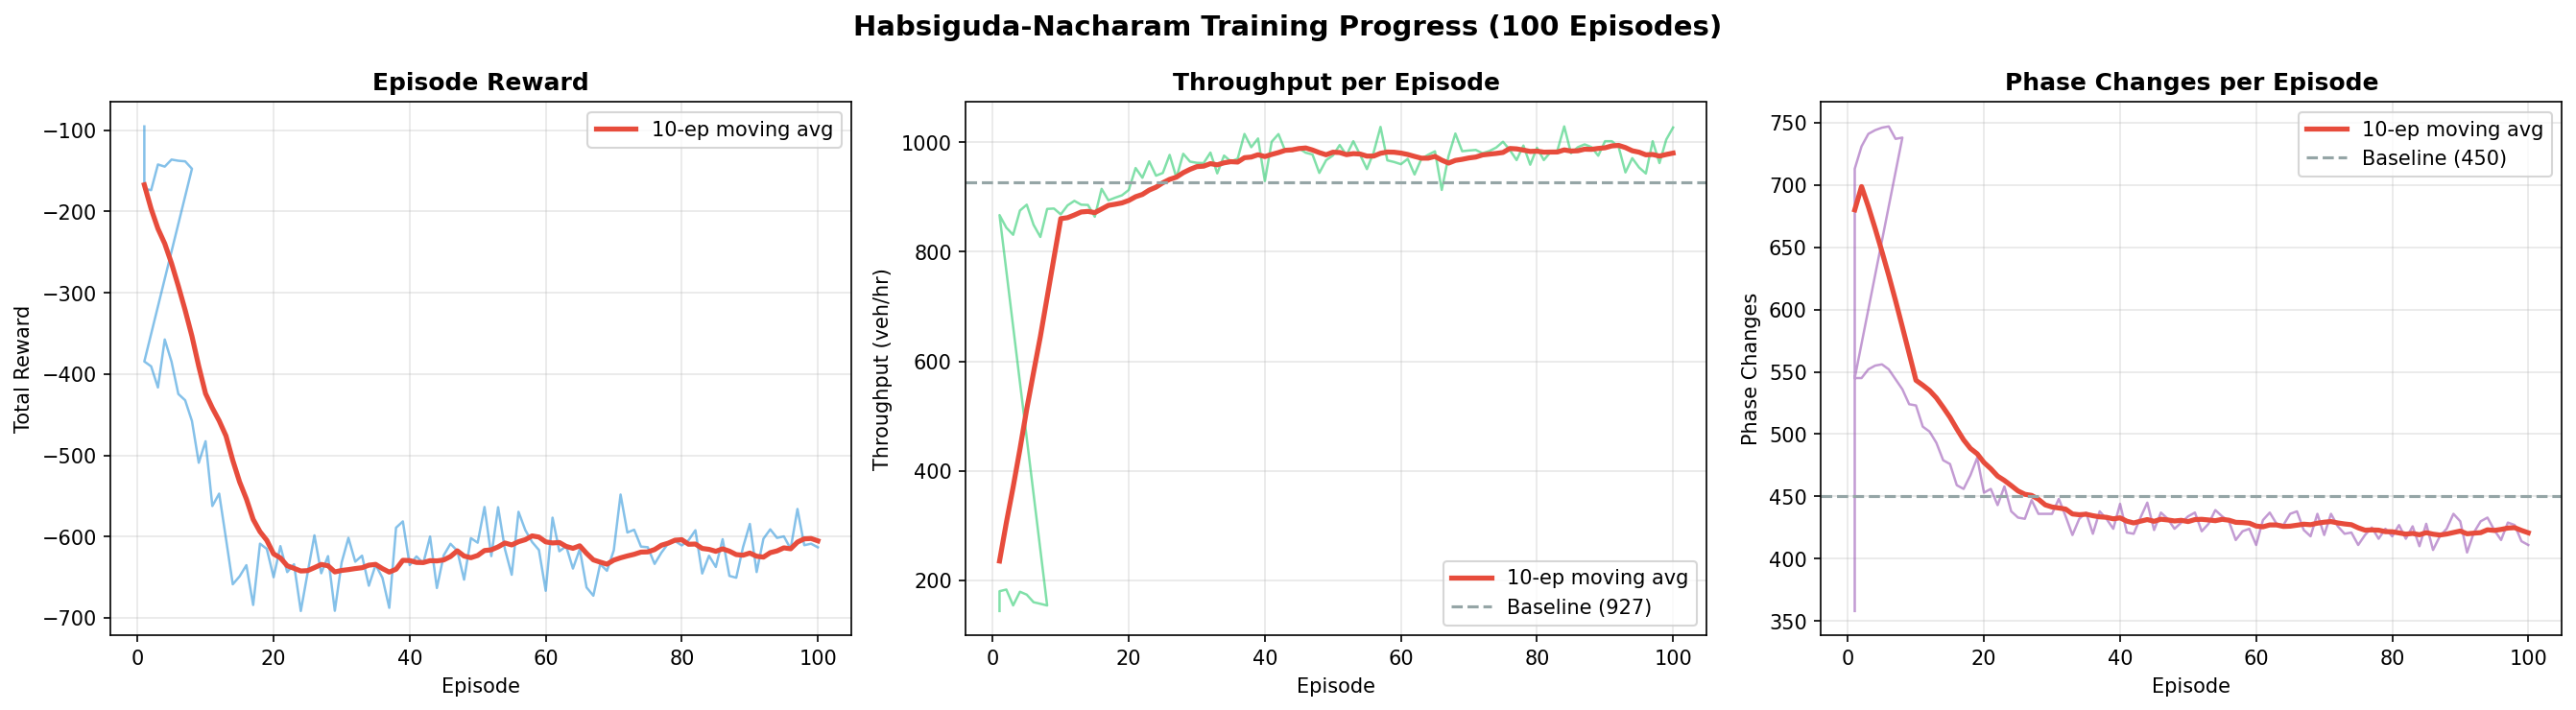
\includegraphics[width=6.8in]{training_curves.png}
\caption{Training on the real-world corridor over 100 fine-tuning episodes
(Stage~5): episode reward (left), throughput against the baseline
(center), and phase changes per episode (right).}
\label{fig:training_hab}
\end{figure*}

\subsection{Evaluation Results}

The fine-tuning pays off. The tuned MH-DQN cuts waiting time by 40.2\%
(1.9\,s vs.\ 3.1\,s) and queue length by 28.2\%, while average speed rises
by 5.1\%. Most importantly, throughput now drops by only 11.0\%, a
three-fold improvement over Stage~4's 33.0\% loss -- and we got there just
by reshaping the reward, without touching the network itself.

\begin{table}[!t]
\caption{Fine-Tuned MH-DQN vs.\ Fixed-Time
         (Stage~5, Real-World Corridor)\label{tab:results_hab}}
\centering
\renewcommand{\arraystretch}{1.2}
\begin{tabular}{@{}lccc@{}}
\toprule
\textbf{Metric} & \textbf{Fixed} & \textbf{MH-DQN} & \textbf{Change} \\
\midrule
Throughput (veh/hr) & 926.7 & 824.4           & $-11.0\%$ \\
Vehicles Completed  & 927.0 & 824.4           & $-11.1\%$ \\
Avg Wait Time (s)   & 3.1   & $\mathbf{1.9}$  & $\mathbf{-40.2\%}$ \\
Avg Queue Length    & 77.0  & $\mathbf{55.3}$ & $\mathbf{-28.2\%}$ \\
Avg Speed (m/s)     & 7.3   & $\mathbf{7.7}$  & $\mathbf{+5.1\%}$ \\
Phase Changes       & 450.0 & 553.2           & $+22.9\%$ \\
\bottomrule
\end{tabular}
\end{table}

% ------------------------------------------------------------------
% FIGURE 17 — Evaluation bar chart Stage 5
% IMAGE: comparison_finetuned.png
% ------------------------------------------------------------------
\begin{figure}[!t]
\centering
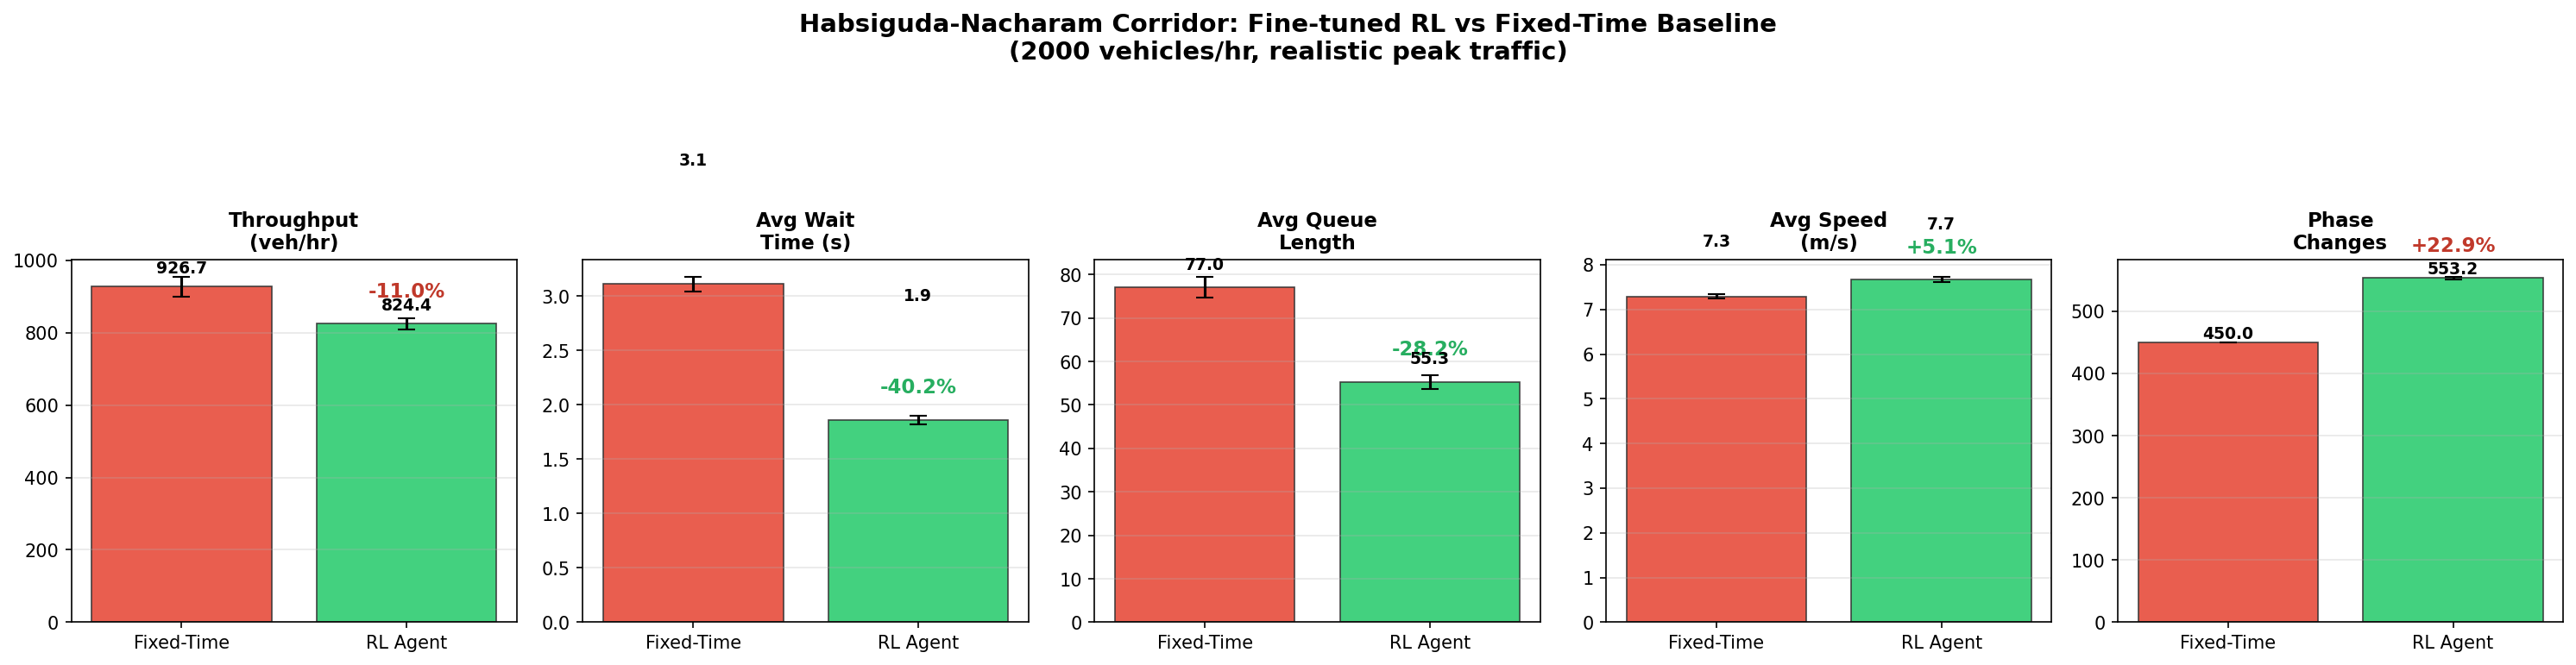
\includegraphics[width=3.4in]{comparison_finetuned.png}
\caption{The fine-tuned MH-DQN compared to the fixed-time baseline on the
real-world corridor (Stage~5, 2{,}000~veh/hr).}
\label{fig:comparison_hab}
\end{figure}

% ------------------------------------------------------------------
% FIGURE 18 — Per-episode comparison Stage 5
% IMAGE: per_episode_comparison.png
% ------------------------------------------------------------------
\begin{figure}[!t]
\centering
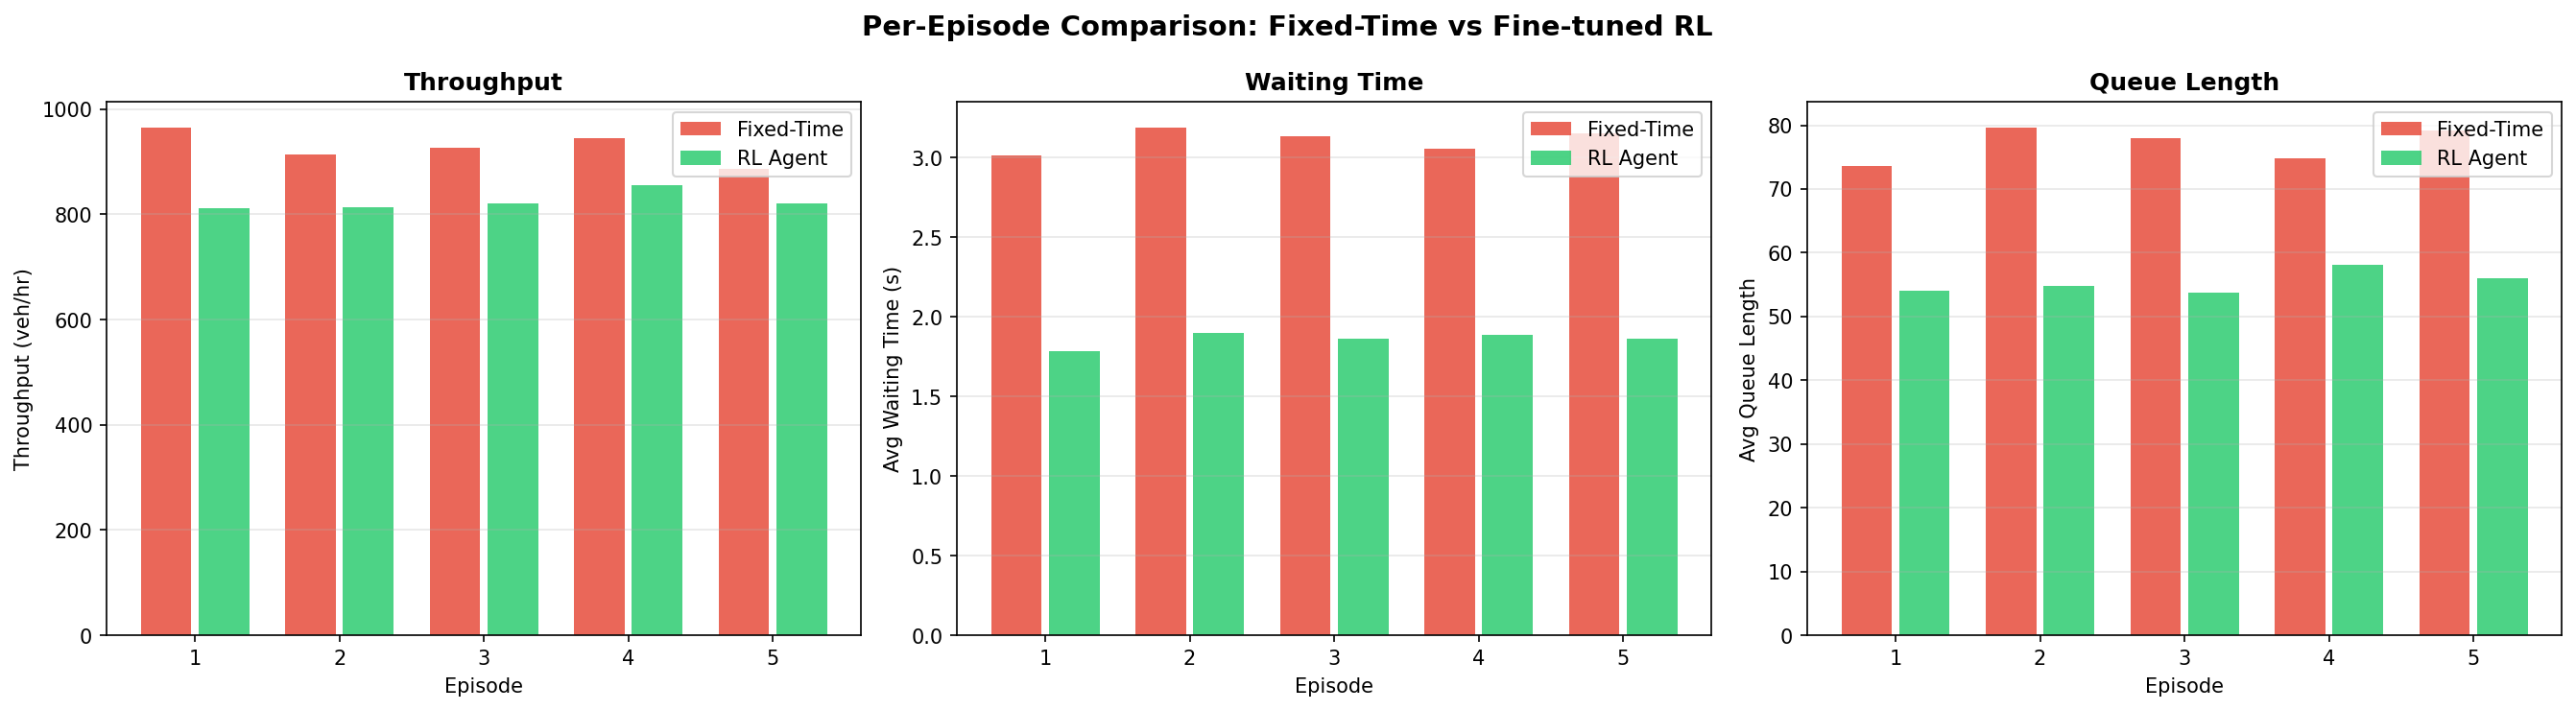
\includegraphics[width=3.4in]{per_episode_comparison.png}
\caption{How performance compares episode by episode over 5 evaluation
episodes on the real-world corridor (Stage~5).}
\label{fig:episodes_hab}
\end{figure}

\subsection{Junction-Level Analysis}

Breaking the reward down by junction at episode~100: J0 ($-127.1$), J1
($-96.3$), J2 ($-113.9$), J3 ($-102.8$), J4 ($-95.3$), J5 ($-73.4$). The
lower penalties at J4 and J5 suggest that junctions further downstream
benefit from the demand-smoothing effect of the junctions upstream of them.
By this point, every junction is operating in the high-traffic regime
(queue $\approx 2.1$--$2.2$, wait $\approx 34$--$36$\,s).

% ---------------------------------------------------------------
\section{Cross-Stage Analysis and Discussion}
\label{sec:discussion}
% ---------------------------------------------------------------

\subsection{Consolidated Cross-Stage Results}

Table~\ref{tab:cross} puts the key stages side by side.
Table~\ref{tab:finetuning_impact} zooms in on exactly what fine-tuning
bought us between Stage~4 and Stage~5. Table~\ref{tab:phase_changes} tracks
phase-change behavior, the variable at the center of the whole trade-off.

\begin{table}[!t]
\caption{Cross-Stage Performance vs.\ Fixed-Time Baseline\label{tab:cross}}
\centering
\renewcommand{\arraystretch}{1.2}
\begin{tabular}{@{}lccc@{}}
\toprule
\textbf{Metric} & \textbf{St.~2} & \textbf{St.~4} & \textbf{St.~5} \\
\midrule
Wait Time Reduc.  & $-73.5\%$    & $-49.5\%$    & $-40.2\%$ \\
Queue Reduction   & $-41.7\%$    & $-35.1\%$    & $-28.2\%$ \\
Throughput Gap    & $-12.9\%$    & $-33.0\%$    & $-11.0\%$ \\
Speed Improvement & ---           & ---           & $+5.1\%$ \\
Phase Chg.\ Ratio & $2.32\times$ & $1.57\times$ & $1.23\times$ \\
\bottomrule
\end{tabular}
\end{table}

\begin{table}[!t]
\caption{Fine-Tuning Impact: Stage~4 $\to$ Stage~5%
\label{tab:finetuning_impact}}
\centering
\renewcommand{\arraystretch}{1.2}
\begin{tabular}{@{}lccc@{}}
\toprule
\textbf{Metric} & \textbf{Stage~4} & \textbf{Stage~5} & \textbf{Change} \\
\midrule
Throughput (veh/hr) & 633.3 & 824.4 & $\mathbf{+30.2\%}$ \\
Wait Time (s)       & 1.57  & 1.86  & $-18.5\%$ \\
Queue Length        & 50.03 & 55.34 & $-10.6\%$ \\
Phase Changes       & 705.2 & 553.2 & $\mathbf{-21.6\%}$ \\
\bottomrule
\end{tabular}
\end{table}

\begin{table}[!t]
\caption{Phase Change Behavior Across Stages\label{tab:phase_changes}}
\centering
\renewcommand{\arraystretch}{1.2}
\begin{tabular}{@{}lccc@{}}
\toprule
\textbf{Stage} & \textbf{RL} & \textbf{Baseline} & \textbf{Ratio} \\
\midrule
Stage~2 (single int.)     & 252.9 & 109.0 & $2.32\times$ \\
Stage~4 (direct transf.)  & 705.2 & 450.0 & $1.57\times$ \\
Stage~5 (fine-tuned)      & 553.2 & 450.0 & $1.23\times$ \\
\bottomrule
\end{tabular}
\end{table}

\subsection{Discussion}

\textbf{Throughput trade-off and reward sensitivity.}
It is striking how close the throughput reduction is in Stage~2 ($-12.89\%$)
and Stage~5 ($-11.0\%$) -- two very different network sizes ending up at
almost the same number. That suggests this small remaining gap is baked
into the reward function itself, not an accident of scale. Raising the
phase penalty from $\lambda=0.05$ to $\lambda=1.0$ closed most of the gap,
taking Stage~4's $-33\%$ throughput loss down to $-11\%$ -- recovering
30.2\% of throughput for a cost of just $+0.29$\,s of extra waiting time.
Because that near-identical gap shows up at two very different scales, it
is not something specific to the corridor's geometry; it is a natural
consequence of optimizing mainly for delay. When the reward mostly cares
about emptying queues fast, the agent learns to serve whichever approach is
most congested right now, in short bursts, and that habit trades a little
bit of steady directional flow for lower moment-to-moment delay. The fact
that changing one penalty term shifts the outcome this much, with no change
to the network or the encoder at all, tells us the trade-off comes from how
the reward is shaped, not from any limit on what the network can represent.

\textbf{The more congested the baseline, the bigger the benefit.}
The corridor's fixed-time baseline already has much higher waiting times
than the single intersection (3.1\,s vs.\ 0.92\,s), simply because it faces
more demand and vehicles can spill back across junctions. And it turns out
the MH-DQN saves more time in absolute terms exactly where things are worse:
1.2\,s saved in the corridor versus 0.68\,s at the single intersection. That
is a useful property to have, because the roads that suffer the most delay
in a real network are exactly the crowded, spillback-prone ones -- so this
is where the biggest gains are needed, and it is also where our controller
delivers the most. A controller that gets better as congestion gets worse is
solving the problem where it actually hurts, rather than mostly helping in
the light-traffic cases that a fixed-time signal already handles just
fine.

\textbf{Soft gating makes phase switching more stable.}
The phase-change ratio steadily falls: $2.32\times$ (Stage~2, hard
switching), then $1.57\times$ (Stage~4), then $1.23\times$ (Stage~5). This
matters a great deal in the real world, where every extra switch means more
mechanical wear on the signal hardware and more uncertainty for drivers.
There is also a direct cost to capacity: every phase change forces a
clearance interval where no movement gets a green light at all, so avoiding
a switch reclaims time that would otherwise be spent doing nothing useful.
The fact that this ratio keeps dropping, in step with the introduction of
soft gating and then the stronger penalty, points to a clear explanation:
blending regime-specific policies smoothly, rather than snapping abruptly
from one to another at the classifier's decision boundary, is what keeps the
control sequence stable.

\textbf{Junctions do not need to talk to each other to cooperate well.}
Across Stages~3--5, none of the agents ever communicate with each other
directly, and yet the decentralized MH-DQN still delivers consistent
improvements -- coordination emerges implicitly, just through the shared
traffic dynamics and the demand-smoothing that upstream junctions naturally
provide to the ones downstream. That is a genuinely useful property for
real-world deployment, since a fully centralized alternative would need
reliable, low-latency communication between every junction and would create
a single point of failure for the whole corridor. A decentralized design
fails much more gracefully: each agent keeps acting on its own local
information even if a neighboring controller goes offline, while still
benefiting from whatever demand-smoothing its upstream neighbors provide.

\textbf{Transfer learning lets the corridor adapt quickly.}
Remarkably, even before any corridor-specific fine-tuning, Stage~4's direct
transfer already achieves $-49.5\%$ waiting time and $-35.1\%$ queue length
on the real corridor. That a policy trained on one synthetic intersection
carries over usefully to a real six-junction corridor tells us the shared
encoder is picking up on demand patterns that hold true regardless of
network size. Fine-tuning then only has to do light specialization work
rather than retrain the model from the ground up, which is exactly where
transfer learning earns its keep: most of the hard representational learning
happens once and gets reused, and adapting to a brand-new site becomes a
short, careful refinement instead of a full training run.

% ---------------------------------------------------------------
\section{Future Work}
\label{sec:future}
% ---------------------------------------------------------------

This step-by-step development suggests several natural next steps:

\begin{enumerate}
    \item \textit{Reward function tuning:} finding a reward that balances
          waiting time and throughput more evenly could shrink the
          remaining $\approx\!11\%$ throughput gap.
    \item \textit{Explicit multi-agent coordination:} letting junctions
          actually talk to each other, through graph neural networks or
          attention mechanisms, could unlock corridor-level coordination
          without giving up the waiting-time gains we already have.
    \item \textit{Hierarchical policy learning:} adding a corridor-level
          policy that oversees the individual junction agents could capture
          benefits that go beyond optimizing each junction on its own.
    \item \textit{Dynamic regime thresholds:} letting the boundaries between
          low, medium, and high regimes adapt on their own could make the
          system more robust across different cities and times of day.
    \item \textit{Real-world deployment:} the next big step is moving these
          SUMO-trained policies onto real intersections, dealing with live
          sensor noise, communication delays, and safety constraints along
          the way.
    \item \textit{Extended corridor networks:} building on what Stage~3
          showed about scalability, the framework could be extended
          city-wide using hierarchical or federated multi-agent methods.
\end{enumerate}

% ---------------------------------------------------------------
\section{Conclusion}
\label{sec:conclusion}
% ---------------------------------------------------------------

This paper has told the story of building a Traffic-Regime Aware Multi-Head
Deep Q-Network for adaptive traffic signal control, one stage at a time,
from a simple proof-of-concept all the way to a real-world corridor
deployment.

It started with a standard DQN on a single four-way intersection (Stage~1).
Adding regime-specific Q-heads and a dynamic classifier (Stage~2) then cut
waiting time by 73.53\% and queue length by 41.69\%, compared to a
30\,s/30\,s fixed-time baseline. A $3\times3$ grid of nine junctions
(Stage~3) confirmed the approach still holds up with multiple agents.
Transferring the model directly to a real six-junction corridor (Stage~4)
improved waiting time by 49.5\%, but came with a 33\% throughput penalty.
Fine-tuning with a stronger phase-change penalty and a longer minimum green
time (Stage~5) recovered 30.2\% of that lost throughput, leaving us with:
a 40.2\% cut in waiting time, a 28.2\% cut in queue length, a 5.1\% gain in
speed, and only an 11.0\% drop in throughput, all under a peak demand of
2{,}000~veh/hr.

Taken together, these results show that teaching a policy to specialize by
traffic regime keeps paying off as the problem grows -- from a single
intersection, to a grid of nine, to a real, tangled, six-junction road
network -- and that carefully fine-tuning the reward is what makes it
possible to keep both congestion and throughput in check once the system
is deployed for real.

% ---------------------------------------------------------------
\section*{Acknowledgment}
% ---------------------------------------------------------------

The authors gratefully acknowledge the open-source reinforcement learning
and traffic simulation communities. Special thanks to the developers of
PyTorch, NumPy, SUMO, and related scientific computing frameworks.

% ---------------------------------------------------------------
% References
% ---------------------------------------------------------------
\begin{thebibliography}{99}

\bibitem{mnih2015human}
V.~Mnih \textit{et al.},
``Human-level control through deep reinforcement learning,''
\textit{Nature}, vol.~518, no.~7540, pp.~529--533, Feb.\ 2015.

\bibitem{wei2018intellilight}
H.~Wei, G.~Zheng, H.~Yao, and Z.~Li,
``IntelliLight: A reinforcement learning approach for intelligent traffic
light control,''
in \textit{Proc.\ ACM SIGKDD Int.\ Conf.\ Knowl.\ Discovery Data Mining},
2018, pp.~2496--2505.

\bibitem{chu2020multiagent}
T.~Chu, J.~Wang, L.~Cod\`{e}ca, and Z.~Li,
``Multi-agent deep reinforcement learning for large-scale traffic signal
control,''
\textit{IEEE Trans.\ Intell.\ Transp.\ Syst.}, vol.~21, no.~3,
pp.~1086--1095, Mar.\ 2020.

\bibitem{hasselt2016deep}
H.~van~Hasselt, A.~Guez, and D.~Silver,
``Deep reinforcement learning with double Q-learning,''
in \textit{Proc.\ AAAI Conf.\ Artif.\ Intell.}, 2016, pp.~2094--2100.

\bibitem{wang2016dueling}
Z.~Wang, T.~Schaul, M.~Hessel, H.~van~Hasselt, M.~Lanctot, and N.~de~Freitas,
``Dueling network architectures for deep reinforcement learning,''
in \textit{Proc.\ Int.\ Conf.\ Mach.\ Learn.}, 2016, pp.~1995--2003.

\bibitem{jacobs1991adaptive}
R.~A.~Jacobs, M.~I.~Jordan, S.~J.~Nowlan, and G.~E.~Hinton,
``Adaptive mixtures of local experts,''
\textit{Neural Comput.}, vol.~3, no.~1, pp.~79--87, 1991.

\bibitem{liang2019deep}
X.~Liang, X.~Du, G.~Wang, and Z.~Han,
``A deep reinforcement learning network for traffic light cycle control,''
\textit{IEEE Trans.\ Veh.\ Technol.}, vol.~68, no.~2,
pp.~1243--1253, Feb.\ 2019.

\bibitem{mannion2018transfer}
P.~Mannion, J.~Duggan, and E.~Howley,
``Transfer learning for multi-intersection traffic signal control,''
in \textit{Proc.\ Int.\ Conf.\ Auton.\ Agents Multiagent Syst.},
2018, pp.~1778--1780.

\bibitem{lopez2018microscopic}
P.~A.~Lopez \textit{et al.},
``Microscopic traffic simulation using SUMO,''
in \textit{Proc.\ IEEE Int.\ Conf.\ Intell.\ Transp.\ Syst.},
2018, pp.~2575--2582.

\bibitem{schaul2016prioritized}
T.~Schaul, J.~Quan, I.~Antonoglou, and D.~Silver,
``Prioritized experience replay,''
in \textit{Proc.\ Int.\ Conf.\ Learn.\ Represent.}, 2016, pp.~1--21.

\bibitem{wei2019presslight}
H.~Wei \textit{et al.},
``PressLight: Learning max pressure control to coordinate traffic signals
in arterial networks,''
in \textit{Proc.\ ACM SIGKDD Int.\ Conf.\ Knowl.\ Discovery Data Mining},
2019, pp.~1290--1298.

\bibitem{haydari2022deep}
A.~Haydari and Y.~Yilmaz,
``Deep reinforcement learning for intelligent transportation systems:
A survey,''
\textit{IEEE Trans.\ Intell.\ Transp.\ Syst.}, vol.~23, no.~1,
pp.~11--32, Jan.\ 2022.

\end{thebibliography}

% ---------------------------------------------------------------
% Author Biographies
% ---------------------------------------------------------------
\vspace{11pt}

\begin{IEEEbiographynophoto}{Suraj Meruva}
(Student Member, IEEE) is pursuing his studies in the Department of Data
Science and Artificial Intelligence at the Indian Institute of Information
Technology, Naya Raipur, Chhattisgarh, India.

His research interests include deep reinforcement learning, intelligent
transportation systems, and multi-agent systems.
\end{IEEEbiographynophoto}

\begin{IEEEbiographynophoto}{Boini Abhiram}
(Student Member, IEEE) is pursuing his studies in the Department of Data
Science and Artificial Intelligence at the Indian Institute of Information
Technology, Naya Raipur, Chhattisgarh, India.

His research interests include reinforcement learning, traffic simulation,
and urban computing.
\end{IEEEbiographynophoto}

\vfill

\end{document}